% LUT core-module ablation table: math, cost and the 21 results (final_val_bpb from each run folder's committed summary.json).
% Build: latexmk -pdf -interaction=nonstopmode -halt-on-error lut_ablation_table_v4.tex
\documentclass[10pt]{article}
\usepackage[landscape,margin=0.55in]{geometry}
\usepackage{lmodern}
\usepackage[T1]{fontenc}
\usepackage{amsmath,amssymb}
\usepackage{booktabs,longtable,array,colortbl}
\usepackage{xcolor}
\usepackage[hang,flushmargin]{footmisc}
\usepackage{pgfplots}\pgfplotsset{compat=1.18}
\usepackage{hyperref}
\hypersetup{colorlinks=true,linkcolor=black,urlcolor=blue}

\newcommand{\tbd}[1]{\textcolor{red!70!black}{\textbf{TBD}~--- #1}}
% \code{...}: typewriter, with a line-break opportunity after every underscore (long class names)
\newcommand{\code}[1]{{\renewcommand{\_}{\textunderscore\allowbreak}\texttt{#1}}}
\newcommand{\sgn}{\operatorname{sgn}}
\newcommand{\note}[1]{\textsuperscript{\textbf{#1}}}
\renewcommand{\arraystretch}{1.25}
\setlength{\LTpre}{4pt}\setlength{\LTpost}{4pt}

\title{LUT core-module ablation: three generations of lookup math\\[2pt]
\large Comparison table}
\date{2026-09-14}
\author{}

\begin{document}
\maketitle
\vspace{-2.5em}

\section*{Protocol}
\textbf{Architecture:} LUT transformer, $E=384$, 6 layers, 6 attention heads. FFN = \code{CompressionMultiHeadLUT} with $H=4$ heads $\times$ $tph=128$ tables
($P=H\cdot tph=512$ tables per token), $d_{in}=d_{out}=48$, $n=8$ anchor pairs per table ($K=2^n=256$ cells); \code{compress} $384\to192$, \code{decompress} $192\to384$.
The vanilla baseline (Table B row V) replaces this FFN with the standard dense one, $384\to1536\to384$, GELU, no bias.
\textbf{Training:} 16{,}000 steps, batch size 48 (24576 tokens), untied embeddings, LUT tables without weight decay.
\textbf{Eval:} validation bits per byte (bpb), \code{evaluate\_bpb\_fixed}, 48 sequences $\times$ 100 steps, first 12 sequences skipped.


\section*{Counting convention}
\begin{itemize}\setlength\itemsep{0pt}
\item Core LUT only, per token, one layer. The \code{compress}/\code{decompress} projections are identical in every row and excluded (147,456 MACs at eval).
\item Row V has no LUT and no projections, so its figures are the whole dense FFN ($E\to4E\to E$, $E=384$); compare them with a LUT row plus the projections. Its 1,536 GELUs are not decomposed into FLOPs.
\item \textbf{FLOP} = one scalar float operation ($+,-,\times,\div$, a comparison, $|\cdot|$, $\exp$, $\log\sigma$, $\sigma$). \textbf{MAC} = a multiply accumulated into a sum; 1 MAC = 2 FLOPs,
  included in the FLOP column. Memory reads and integer work are not counted.
\item \textbf{Eval} = exactly what inference computes, per token. \textbf{Train} = the whole cost of one training step: the computation training shares with inference, all gradients, including per-table gradients of per-layer scalars,
  and anything computed only in training --- a score or blend weight the eval read does not use, and a surrogate's score, blend weights and gradients (not the surrogate's value, note b).
  A hard-forward row's eval is therefore the hard read alone, while its train adds the surrogate. Train $=$ eval $+$ the training-only work, except for row 3.2 int8 (note d).
\end{itemize}

\newpage
\section*{Table A --- forward function and gradient function}
Per variant, (a) is the function computed on the forward pass and (b) the function whose gradient training uses: the weights always receive the gradient of (a),
while the input, the temperatures and the learned per-layer scalars receive the gradient of (b) with the table weights held constant.
\footnotesize
\arrayrulecolor{black!45}\setlength{\extrarowheight}{1.5pt}%
\newcommand{\spanab}[1]{\multicolumn{2}{>{\raggedright\arraybackslash}p{\dimexpr 20.8cm+2\tabcolsep+\arrayrulewidth\relax}|}{#1}}%
\newcommand{\genrow}[1]{\multicolumn{3}{|l|}{#1}}%
\begin{longtable}{|>{\raggedright\arraybackslash}p{2.9cm}|>{\raggedright\arraybackslash}p{10.2cm}|>{\raggedright\arraybackslash}p{10.6cm}|}
\hline
\textbf{Variant} & \textbf{(a) Forward: the function computed} & \textbf{(b) Backward: the function whose gradient is used} \\
\hline
\endfirsthead
\hline
\textbf{Variant} & \textbf{(a) Forward: the function computed} & \textbf{(b) Backward: the function whose gradient is used} \\
\hline
\endhead
\multicolumn{3}{r}{\emph{continued on next page}} \\
\endfoot
\hline
\endlastfoot

\genrow{\textbf{GEN 1 --- Spiking Manifesto basic model}} \\ \hline
1.1 Hard forward, two-alternatives backward &
$y=\sum_tW_t[c_t]$, summed over tables $t$: each of table $t$'s $n$ anchor pairs gives a signed margin $u_j=z[a_j]-z[b_j]$; the $n$ signs $[u_j>0]$ are the bits of the binary index $c_t\in\{0,\dots,2^n-1\}$ of the row read from $W_t\in\mathbb R^{K\times d}$, $K=2^n$. &
The 2-cell blend $\sum_t\big[(1-U_t)W_t[c_t]+U_tW_t[c_t']\big]$, $U_t=U(u_{j^\star})$, $U(u)=0.5/(1+|u|)$, with the least-confident pair $j^\star=\arg\min_j|u_j|$ and $c'$ ($c$ with bit $j^\star$ flipped) held fixed.
The pairing with (a) is exact as a stop-gradient composite; the blend is $C^1$ across a bit flip and jumps only where $j^\star$ switches. \\[2pt] \hline
1.2 Soft forward, two-alternatives backward &
\spanab{\textbf{(a) = (b):} the blend of 1.1(b), applied at eval too.} \\[2pt] \hline
\genrow{\textbf{GEN 2 --- FastMHL math}} \\ \hline
2.1 Hard forward, all-alternatives backward (all $K$ cells) &
$y=\sum_tW_t[c_t]$, as 1.1(a). &
With $b_j(\ell)=+1$ if the bit of $\ell$ for pair $j$ is 1, else $-1$, and the squashed margin $\hat m_j=u_j/(T_s+|u_j|)\in(-1,1)$: $s_\ell=\sum_jb_j(\ell)\,\hat m_j$ scores how well row $\ell$'s bit pattern agrees with the actual signs of the margins (small margins count little either way).
All $K$ rows of each table are read, softmax-weighted within that table: $\sum_t\sum_{\ell<K}\mathrm{softmax}_\ell(s_\ell/T_{sel})\,W_t[\ell]$.
$T_s,T_{sel}$: per-layer learned scalars.
Globally $C^1$ in the input; never uses the address, whose row is the one with the largest weight. \\[2pt] \hline
2.2 Hybrid\_smooth two-alternatives forward, all-alternatives backward &
Reads two cells, the addressed $c_t$ and the alternative $c_t'$ ($c_t$ with the bit of the least-confident pair $j^\star=\arg\min_j|u_j|$ flipped), blended by a weight set by that pair's margin:
$y=\sum_t\big[(1-w_t)W_t[c_t]+w_tW_t[c_t']\big]$, $w_t=\sigma(-2\rho_{j^\star}/T_{sel})\in(0,\tfrac12]$, $\rho_j=|u_j|/(T_s+|u_j|)$, $\sigma$ the logistic sigmoid; applied at eval too. &
The same softmax-weighted read of all $K$ rows as 2.1(b), with the same $T_s,T_{sel}$ parameters as (a). \\[2pt] \hline
2.3 Hard forward, 2-alternatives backward &
The hard read of 1.1(a). &
The softmax of 2.1(b) restricted to the two cells $c_t$ and $c_t'$ ($c_t$ with the bit of the least-confident pair $j^\star=\arg\min_j|u_j|$ flipped) and renormalised over that pair.
The weight on $c_t'$ is $\sigma(-2\rho_{j^\star}/T_{sel})$, $\rho_j=|u_j|/(T_s+|u_j|)$, $\sigma$ the logistic sigmoid: exactly 2.2(a)'s $w_t$, so this is 2.2(a)'s 2-cell blend. \\[2pt] \hline
2.4 Hybrid\_smooth two-alternatives forward, 2-alternatives backward &
\spanab{\textbf{(a) = (b):} the 2-cell blend of 2.2(a). The backward keeps only 2 of the $K$ rows, the addressed $c_t$ and its least-confident neighbour $c_t'$, which are exactly the two cells the forward reads,
so the restricted softmax equals the forward weight $w_t$ and forward and backward coincide; unlike 2.2, the input gradient reaches only pair $j^\star$.} \\[2pt] \hline
\genrow{\textbf{GEN 3 --- LightMHL math (LookupFFN-inspired): learned margin score}} \\ \hline
\textbf{3.1 The Gen-3 form:} learned margin score, one cell, per-layer $(\beta,\gamma)$ &
\spanab{\textbf{(a) = (b):} $y=\sum_t s_tW_t[c_t]$ with the address $c_t$ held fixed; $s_t=S_tP_t^{\gamma}$, $S_t=\sum_jm_j$, $P_t=\prod_j\sigma(\beta m_j)$, $m_j=|u_j|$, computed as $S_t\exp\!\big(\gamma\sum_j\log\sigma(\beta m_j)\big)$;
$\beta,\gamma$ learned per layer from $(2,1)$, where $s_t$ is LookupFFN's margin score. Discontinuous at cell boundaries, since $\sigma(0)>0$.} \\[2pt] \hline
3.2 The Gen-3 form, two alternatives, per-layer $(\beta,\gamma,\tau)$ &
\spanab{\textbf{(a) = (b):} each table reads two cells, $y=\sum_t s_t\big[(1-v_t)W_t[c_t]+v_tW_t[c_t']\big]$, with $s_t$ as in 3.1 over all $n$ margins and $c_t'$ the cell $c_t$ with the bit of the smallest margin $j^\star=\arg\min_jm_j$ flipped ($c_t,c_t',j^\star$ held fixed).
$v_t$ is a softmax over the two cells with logits $0$ and $-2m_{j^\star}/\tau$ (flipping bit $j$ lowers $\langle u,b\rangle$ by $2m_j$), i.e.\ $v_t=\sigma(-2m_{j^\star}/\tau)\in(0,\tfrac12]$; $\tau$ learned per layer from $0.5$.
The input gradient reaches all $n$ margins through $s_t$ and $m_{j^\star}$ alone through $v_t$. Continuous across a bit flip ($v_t=\tfrac12$ there); jumps where $j^\star$ switches.} \\[2pt] \hline
3.3 / 3.4 Hard forward, Gen-3 backward (3.1 / 3.2) &
The hard read of 1.1(a), $y=\sum_tW_t[c_t]$; no score at eval. &
3.1(b) (for 3.3) or 3.2(b) (for 3.4) on detached weights, with each score divided by the detached mean score of its head ($\hat s_t=s_t/\mathrm{sg}(\bar s+\epsilon)$), which keeps these gradients bounded (without it training diverged, \code{b5b0f2c3}); the weights get (a)'s gradient.
Kept as evidence that a hard forward is weak, not as candidates. \\[2pt]
\end{longtable}
\arrayrulecolor{black}\setlength{\extrarowheight}{0pt}
\normalsize

\section*{Table B --- cost and results}
Per token, one layer, core LUT only (row V: the whole dense FFN); $P=512$, $H=4$, $n=8$, $K=256$, $d=48$, $E=384$.
\textbf{Validation bpb:} \code{final\_val\_bpb} from the committed \code{summary.json} of the cell's run folder \code{abl\_NN} in \code{experiments/ffn\_replacement/lut\_ablation}, one seed each; in parentheses the difference from V (1.165148).
Two vanilla seeds at 16K differ by 0.00335 (\code{exp\_n\_0135} 1.165147, \code{exp\_n\_0176} 1.161798), so smaller differences are inside single-seed noise.
\footnotesize
\setlength{\tabcolsep}{3pt}% eight columns: narrower gutters keep the table inside the text block
\begin{longtable}{>{\raggedright\arraybackslash}p{1.3cm} >{\raggedright\arraybackslash}p{2.8cm} >{\raggedright\arraybackslash}p{4.2cm} >{\raggedright\arraybackslash}p{2.0cm} >{\raggedright\arraybackslash}p{2.8cm} >{\raggedright\arraybackslash}p{2.5cm} >{\raggedright\arraybackslash}p{2.5cm} >{\raggedright\arraybackslash}p{4.9cm}}
\toprule
\textbf{Variant} & \textbf{Eval FLOPs} & \textbf{Train FLOPs} & \textbf{Eval MACs} & \textbf{Train MACs} & \textbf{Validation bpb} & \textbf{Validation bpb, $+$TV ($\lambda=10$)} & \textbf{Implementation (class used)} \\
\midrule
\endfirsthead
\toprule
\textbf{Variant} & \textbf{Eval FLOPs} & \textbf{Train FLOPs} & \textbf{Eval MACs} & \textbf{Train MACs} & \textbf{Validation bpb} & \textbf{Validation bpb, $+$TV ($\lambda=10$)} & \textbf{Implementation (class used)} \\
\midrule
\endhead
\midrule \multicolumn{8}{r}{\emph{continued on next page}} \\
\endfoot
\bottomrule
\endlastfoot
V &
$2\cdot2E\cdot4E=\mathbf{2{,}359{,}296}$ $+$ 1,536 GELUs &
$2\cdot2E\cdot4E+2\cdot4E\cdot4E+4E=\mathbf{7{,}079{,}424}$ $+$ 1,536 GELUs, 1,536 GELU$'$ &
$2E\cdot4E$ $=\mathbf{1{,}179{,}648}$ &
$2E\cdot4E+4E\cdot4E=\mathbf{3{,}538{,}944}$ &
\textbf{1.165148}, \code{abl\_10}; parent \code{exp\_n\_0135} 1.165147; seed 2 1.161798 (\code{exp\_n\_0176}) &
n/a: no LUT tables &
Dense FFN (\code{ffn\_type='dense'}): \code{Linear(384, 1536, bias=False)}, GELU, \code{Linear(1536, 384, bias=False)}. \\
\midrule
1.1 &
$P(2n+d)=\mathbf{32{,}768}$ &
$P(6d+4n+9)=\mathbf{168{,}448}$ &
$0$ &
$P\cdot2d=\mathbf{49{,}152}$ &
\textbf{1.199672} ($+0.0345$), \code{abl\_11} &
\textbf{1.193616} ($+0.0285$), \code{abl\_12} &
\code{CompressionMultiHeadLUT(lut\_impl='gen1')}: \code{MultiHeadLut(smooth\_mode=False, n\_alternatives=1, uncertainty\_mode=INVERSE\_L1, weights\_init='uniform')}, each head's anchors in its own slice. \\
1.2 &
$P(4d+4n+4)=\mathbf{116{,}736}$ &
$P(12d+4n+13)=\mathbf{317{,}952}$ &
$P\cdot2d=\mathbf{49{,}152}$ &
$P\cdot6d=\mathbf{147{,}456}$ &
\textbf{1.185924} ($+0.0208$), \code{abl\_13} &
\textbf{1.181644} ($+0.0165$), \code{abl\_14} &
As 1.1 with \code{smooth\_mode=True}. \\
\midrule
2.1 &
$P(2n+d)=\mathbf{32{,}768}$ &
$P(2Kd+4nK+9K+13n+2d)$ $=\mathbf{18{,}059{,}264}$\note{a} &
$0$ &
$P(Kd+2nK)$ $=\mathbf{8{,}388{,}608}$ &
\textbf{1.181035} ($+0.0159$), \code{abl\_07}; parent \code{exp\_n\_0121} 1.180622 &
\textbf{1.174661} ($+0.0095$), \code{abl\_15} &
\code{FastMultiHeadLut(forward\_mode='hard', backward\_topk=0)}. \\
2.2 &
$P(2kd+4n+5)=\mathbf{117{,}248}$, $k=2$ cells read &
$P(2Kd+4nK+9K+15n+4kd+5)$ $=\mathbf{18{,}217{,}472}$\note{a} &
$P\,kd=\mathbf{49{,}152}$ &
$P(Kd+2nK+2kd)$ $=\mathbf{8{,}486{,}912}$ &
\textbf{1.169401} ($+0.0043$), \code{abl\_01} &
\textbf{1.162635} ($-0.0025$), \code{abl\_16} &
\code{FastMultiHeadLut(forward\_mode='hybrid\_smooth', backward\_topk=0)}. \\
2.3 &
$P(2n+d)=\mathbf{32{,}768}$ &
$P(2kd+4nk+9k+14n+2d-1)$ $=\mathbf{246{,}272}$, $k=2$ cells &
$0$ &
$P(kd+2nk)=\mathbf{65{,}536}$ &
\textbf{1.203803} ($+0.0387$), \code{abl\_02} &
\textbf{1.196908} ($+0.0318$), \code{abl\_17} &
\code{FastMultiHeadLut(forward\_mode='hard', backward\_topk=1)}; \code{backward\_topk} counts the cells kept besides $c_t$. \\
2.4 &
$P(2kd+4n+5)=\mathbf{117{,}248}$ &
$P(6kd+13n+20)=\mathbf{358{,}400}$ &
$P\,kd=\mathbf{49{,}152}$ &
$P\,3kd=\mathbf{147{,}456}$ &
\textbf{1.179331} ($+0.0142$), \code{abl\_03} &
\textbf{1.174482} ($+0.0093$), \code{abl\_18} &
\code{FastMultiHeadLut(forward\_mode='hybrid\_smooth', backward\_topk=1)}. \\
\midrule
\textbf{3.1} &
$P(2kd+7n+1)=\mathbf{78{,}336}$, $k=1$\note{b} &
$P(6kd+17n+9)=\mathbf{221{,}696}$\note{b} &
$P\,kd=\mathbf{24{,}576}$ &
$P\,3kd=\mathbf{73{,}728}$ &
\textbf{1.169578} ($+0.0044$), \code{abl\_08}; parent \code{exp\_g\_0248} 1.169328 &
\textbf{1.163849} ($-0.0013$), \code{abl\_09}; parent \code{exp\_g\_0249} 1.163698 &
\code{LightMultiHeadLUT(confidence\_form='learned\_margin', learned\_margin\_init=(0, 2, 1), learned\_margin\_freeze\_g=True)}, with $g$ the log-gain, held at 0. \\
3.2 &
$P(2kd+8n+8)=\mathbf{135{,}168}$, $k=2$\note{b} &
$P(6kd+18n+31)=\mathbf{384{,}512}$\note{b} &
$P\,kd=\mathbf{49{,}152}$ &
$P\,3kd=\mathbf{147{,}456}$ &
\textbf{1.159969} ($-0.0052$), \code{abl\_04} &
\textbf{1.154739} ($-0.0104$), \code{abl\_05} &
As 3.1 with \code{read\_top\_n=2, read\_tau=0.5, read\_tau\_learnable=True}. \\
3.2 int8 &
$P(7n+16)+Hd=\mathbf{37{,}056}$\note{d} &
$P(6kd+17n+57)=\mathbf{393{,}728}$, $k=2$\note{d} &
$0$ &
$P\,3kd=\mathbf{147{,}456}$ &
not run &
\textbf{1.158890} ($-0.0063$), \code{abl\_48}; unquantised rerun \code{abl\_46} 1.155175 &
As 3.2 with \code{quant\_mode='p2\_int8'}: power-of-two cell weights, int8 cells (section at the end). \\
3.3 &
$P(2n+d)=\mathbf{32{,}768}$ &
$P(4d+17n+11)+H=\mathbf{173{,}572}$\note{b} &
$0$ &
$P\,d=\mathbf{24{,}576}$ &
\textbf{1.210356} ($+0.0452$), \code{abl\_19} &
\textbf{1.198918} ($+0.0338$), \code{abl\_20} &
As 3.1, hard forward.\note{c} \\
3.4 &
$P(2n+d)=\mathbf{32{,}768}$ &
$P(6d+18n+32)+H=\mathbf{237{,}572}$\note{b} &
$0$ &
$P\,2d=\mathbf{49{,}152}$ &
\textbf{1.201621} ($+0.0365$), \code{abl\_21} &
\textbf{1.196248} ($+0.0311$), \code{abl\_22} &
As 3.2, hard forward.\note{c} \\
\end{longtable}
\normalsize
\begingroup\makeatletter\@beginparpenalty=\@M\makeatother% keep the heading with its first note
\noindent\textbf{Notes to Table B.}\par\nopagebreak
\begin{itemize}\setlength\itemsep{0pt}\footnotesize
\item[\note{a}] Dominated by $2Kd$: every table's $K$ rows are read; several \code{[tokens, 512, 256]} fp32 buffers of about 12.9\,GiB at 24,576 tokens.
\item[\note{b}] Per table, eval: $n$ comparisons, $n$ differences, $n$ absolute values, $n$ products $\beta m_j$, $n$ $\log\sigma$, the two sums, $\times\gamma$, $\exp$ and the final product ($7n+1$), plus the scaled rows ($2kd$);
  3.2 adds the argmin ($n-1$), the logit $-2m_{j^\star}/\tau$ (2), the two-way softmax (4) and $s_t$ times the two weights (2).
  Train adds, as training-only work: the row terms ($4kd$), the input term ($8n+3$) and the per-table accumulation of the parameter gradients ($\partial\log\gamma$ 3, $\partial\log\beta$ $2n+2$);
  3.2 adds $\partial s_t$ from two rows (3), $\partial v_t$ (2), the softmax gradient (5), $\partial m_{j^\star}$ (3) and $\partial\log\tau$ (2).
  The parameter gradients are scalar multiplies, so they add no MACs.
  3.3, 3.4: inference performs the hard read alone, while training also reads a surrogate on detached weights (3.1's / 3.2's read with the score rescale).
  In the count, eval is the hard read; train adds the surrogate's score (and for 3.4 the argmin and two-way softmax) and the score rescale ($+2P+H$ / $+3P+H$ FLOPs, no MACs),
  with each row's score-scaled weight update replaced by one plain update at $c_t$: training-only work $P(3d+15n+9)+2P+H=140{,}804$ (3.3) and $P(5d+16n+29)+3P+H=204{,}804$ (3.4).
  Not counted: the value of the surrogate $f$ and the $+f-\mathrm{sg}(f)$ pair, which cancel exactly (the implementation evaluates them).
  \textbf{Training-only work} (train $-$ eval), FLOPs / MACs, so the gradient cost can be read in isolation: V $4{,}720{,}128$ $+$ 1,536 GELU$'$ / $2{,}359{,}296$; 1.1 $135{,}680$ / $49{,}152$; 1.2 $201{,}216$ / $98{,}304$;
  2.1 $18{,}026{,}496$ / $8{,}388{,}608$; 2.2 $18{,}100{,}224$ / $8{,}437{,}760$; 2.3 $213{,}504$ / $65{,}536$; 2.4 $241{,}152$ / $98{,}304$; 3.1 $143{,}360$ / $49{,}152$; 3.2 $249{,}344$ / $98{,}304$;
  3.2 int8 $356{,}864$ / $147{,}456$ (not train $-$ eval, note d); 3.3 $140{,}804$ / $24{,}576$; 3.4 $204{,}804$ / $49{,}152$.
\item[\note{c}] 3.3, 3.4 run on code with the score rescale (\code{b5b0f2c3}); without it all four diverged (final bpb 2.7--3.2).
\item[\note{d}] 3.2 int8, counted under the same convention as note b (eval = what inference computes, train = the whole training step), with five choices stated.
  \textbf{Eval, per table} (the deployed integer read): $n$ comparisons and $n$ differences (the address), $n$ absolute values, the sum $S$ ($n-1$), $n$ products $\beta m_j$, $n$ $\log\sigma$ and their sum ($n-1$), the argmin ($n-1$) --- $7n-3$, shared with 3.2;
  then $q_t$: $m_{j^\star}$ times the per-layer constant $2/(\tau\ln2)$, $+\tfrac12$, floor, clamp to $[0,J]$ (5); $c_{q_t}$: the test $q_t<C$, $2^{-q_t}$, $+1$, $\log_2$ (4); $k'_t$: $\log_2S_t$, $\times\gamma$, $\div\ln2$, $+$, $-c_{q_t}$, $+\tfrac12$, floor (7);
  the window and drop tests: $k'_t<-3$, $k'_t>4$, $q_t>3$ (3). Total $7n+16$ per table.
  The shifts $k'_t+6$, $k'_t+6-q_t$ and the two-cell shift-add over the int8 cells are integer work, so they count 0 FLOPs and 0 MACs; the one conversion of the $Hd$ int32 accumulators to float per token counts $Hd$.
  \textbf{Training-only work, per table}: the float read of the two cells at their straight-through weights ($2kd$, $kd$ MACs); the score and blend values eval does not form --- $\exp$ and the product $S_t\cdot\exp$ (2), the logit (2), the two-way softmax (4), $s_t$ times the two weights (2);
  the straight-through ratios: $2^{k'_t}$ and $2^{k'_t-q_t}$ as floats (2), the clamp of the two exact weights (2) and the two divisions (2); their use in the gradient, the two multiplies $\partial w\cdot$ratio (2);
  and 3.2's gradients unchanged, $4kd+10n+23$ with $2kd$ MACs. Total $6kd+10n+41$ with $3kd$ MACs, i.e.\ $356{,}864$ FLOPs and $147{,}456$ MACs.
  \textbf{Train} $=$ the per-table integers ($7n+16$, as in eval) $+$ this training-only work $=P(6kd+17n+57)=393{,}728$ FLOPs and $147{,}456$ MACs.
  \textbf{This row is the one exception to train $=$ eval $+$ training-only work} ($37{,}056+356{,}864=393{,}920$): the $Hd=192$ int32$\to$float conversions per token are eval-only ---
  training computes the same per-table integers but then performs the float straight-through read instead of the integer read, so it never converts ($393{,}728=37{,}056-192+356{,}864$).
  \textbf{Choices:} (1) operations outside the FLOP list (floor, $\log_2$, $2^{-q}$) count 1 FLOP each, as $\exp$ and $\log\sigma$ do in note b; $c_{q_t}$ is counted as computed, as the code does --- as a lookup in a $C$-entry table it would cost 0;
  as in note b, the log-gain $g$ (held at 0) is not counted, nor are straight-through value pairs of the form $f-\mathrm{sg}(f)$, which cancel exactly.
  (2) The int32$\to$float conversion counts 1 FLOP per accumulator element ($Hd$ per token), in eval only.
  (3) Worst case: every table read and both cells taken; skipping ($k'_t<-3$) and dropping the second cell ($q_t>3$) make the measured average lower, so these figures are upper bounds (the integer read has no FLOPs to save, but training's float read does).
  (4) The float straight-through read exists only in training and is counted in train, not in eval.
  (5) The per-step table quantisation (per weight: $|\cdot|$, the running max, $\div2^{e_{h,i}}$, $+\tfrac12$, floor, two clamp comparisons, $\times2^{e_{h,i}}$ = 8 FLOPs over $P\,K\,d=6{,}291{,}456$ weights, plus 4 per exponent over $Hd$)
  is training only and is amortised over the 24,576 tokens of a step: $+2{,}048$ FLOPs and no MACs per token per layer. As with the TV penalty, it is stated here and not included in the columns.
\end{itemize}
\endgroup

\noindent\textbf{Hard forward.} With the Gen-3 backward unchanged, replacing the blended forward by the hard read costs $+0.041$ (3.3 vs 3.1), $+0.035$ (3.3 vs 3.1, $+$TV), $+0.042$ (3.4 vs 3.2) and $+0.042$ bpb (3.4 vs 3.2, $+$TV), the same direction as Gens 1--2 (1.1, 2.1, 2.3 against 1.2, 2.2, 2.4): a blending or confidence-weighted forward is necessary. Rows 3.3 and 3.4 are kept for this comparison only.

\section*{Cell TV regularisation (Table B's $+$TV column)}
\begin{itemize}\setlength\itemsep{1pt}
\item \textbf{Penalty:} $\lambda\cdot\frac16\sum_{\text{layers}}\frac{1}{P\,n\,2^{n-1}}\sum_t\sum_{(c,c')}\|W_t[c]-W_t[c']\|^2$, squared L2 over the cell pairs $(c,c')$ that differ in one bit, $\lambda=10$; its gradient is added once per step, before gradient clipping.
  Training only: $+6{,}144$ FLOPs and $+2{,}048$ MACs per token per layer (amortised over 24,576 tokens); inference unchanged.
\item \textbf{All three generations:} the trainer's penalty (\code{lut\_tv\_penalty}) covers \code{MultiHeadLut}, \code{FastMultiHeadLut} and \code{LightMultiHeadLUT} tables, whose Hamming-1 cell pairs were checked through each module's read path,
  and \code{build\_model} refuses $\lambda>0$ on a model whose tables it cannot reach.
\end{itemize}

\section*{Quantised variant of 3.2 $+$TV: power-of-two cell weights and int8 cells}
The best LUT cell, 3.2 $+$TV, is quantised so that the deployed read of a table uses only cell lookups, additions and bit shifts over 8-bit integer cells;
the few per-table scalars that steer it stay in floating point. The notation is Table A's: table $t$ has margins $u_j=z[a_j]-z[b_j]$, $m_j=|u_j|$,
addressed cell $c_t$, alternative cell $c_t'$ (the bit of $j^\star=\arg\min_jm_j$ flipped), score $s_t=S_tP_t^{\gamma}$ and blend weight $v_t=\sigma(-2m_{j^\star}/\tau)$ on $c_t'$;
$T=128$ tables per head, cell width $d=48$. Rounding is $\operatorname{round}(\xi)=\lfloor\xi+\tfrac12\rfloor$ (half up); a multiply by $2^{m}$ is a shift by $m$ bits.
It is implemented as \code{quant\_mode='p2\_int8'} of \code{LightMultiHeadLUT}.

\subsection*{From the blend to shifts and adds}
3.2's read of table $t$ is $s_t\big[(1-v_t)W_t[c_t]+v_tW_t[c_t']\big]$. Three steps turn its two weights into powers of two.
\begin{itemize}\setlength\itemsep{1pt}
\item \textbf{Factorise (exact).} With $r_t=v_t/(1-v_t)=e^{-2m_{j^\star}/\tau}$: \ $s_t\big[(1-v_t)W_t[c_t]+v_tW_t[c_t']\big]=s_t(1-v_t)\big(W_t[c_t]+r_t\,W_t[c_t']\big)$.
\item \textbf{Round $r_t$.} $q_t=\operatorname{clamp}\big(\lfloor 2m_{j^\star}/(\tau\ln2)+\tfrac12\rfloor,0,J\big)$, so $r_t\approx2^{-q_t}$, and $c_{q}=\log_2(1+2^{-q})$ for $q<C$, $0$ otherwise, so $\log_2(1+r_t)\approx c_{q_t}$;
  $J=64$, $C=8$. If $q_t>Q=3$ the second cell's weight is below $1/8$ and it is dropped.
\item \textbf{Round $s_t(1-v_t)$.} Since $\log_2\big(s_t(1-v_t)\big)=\log_2s_t-\log_2(1+r_t)$, set $k'_t=\operatorname{round}(\log_2s_t-c_{q_t})$, with the score in the log domain,
  $\log_2s_t=\log_2S_t+\frac{\gamma}{\ln2}\sum_j\log\sigma(\beta m_j)$, so $P_t$ is never formed.
\item \textbf{Exponent window.} $k'_t\in[-3,4]$ ($L=8$ values): a table with $k'_t<-3$ is skipped, one with $k'_t>4$ is clamped to $4$.
\end{itemize}
Table $t$ then reads $2^{k'_t}\big(W_t[c_t]+2^{-q_t}W_t[c_t']\big)$, or $2^{k'_t}W_t[c_t]$ when the second cell is dropped.

\subsection*{Training and integer cells}
\begin{itemize}\setlength\itemsep{1pt}
\item \textbf{Straight-through cell weights.} Training reads $\hat w_tW_t[c_t]+\hat w'_tW_t[c_t']$ with $\hat w_t=s_t(1-v_t)\,\mathrm{sg}\big(2^{k'_t}/(s_t(1-v_t))\big)$ and
  $\hat w'_t=s_tv_t\,\mathrm{sg}\big(2^{k'_t-q_t}/(s_tv_t)\big)$: in value exactly $2^{k'_t}$ and $2^{k'_t-q_t}$ ($0$ when dropped or skipped), with the gradients of $s_t(1-v_t)$ and $s_tv_t$
  times the same ratios, so $\beta,\gamma,\tau$ and the input keep learning and skipped tables can come back. The trained read is the deployed read.
\item \textbf{Int8 cells.} Each weight is an 8-bit integer times a power of two shared by head $h$ and output channel $i$:
  $e_{h,i}=\big\lceil\log_2\max_{t\in h,\ c}|W_t[c]_i|\big\rceil-7$, $\ \hat W=\operatorname{clamp}\big(\operatorname{round}(W/2^{e_{h,i}}),-128,127\big)$;
  training uses $2^{e_{h,i}}\hat W$ in value with the gradient passed to the float $W$ unchanged, and $e_{h,i}$ is recomputed from $W$ on every forward pass.
\item \textbf{Scales cost nothing at runtime.} Nothing sits between the table sum and \code{decompress}, and $e_{h,i}$ is common to head $h$'s tables, so after training
  $2^{e_{h,i}}$ is multiplied into column $dh+i$ of \code{decompress}'s weight matrix $M$ (once, at export).
\end{itemize}
The deployed head sum, in integers kept in units of $2^{-6}$ so that every shift is a left shift, is
\[
\hat y_h=\sum_{t\in h,\ k'_t\ge-3}\big(\hat W_t[c_t]\ll(k'_t+6)\big)+\big(\hat W_t[c_t']\ll(k'_t+6-q_t)\big),\qquad \text{out}=M'\,[\hat y_1;\dots;\hat y_H]+\text{bias},
\]
the second term left out when $q_t>3$, $M'$ being $M$ with $2^{e_{h,i}-6}$ folded into its columns; $|\hat y_h|\le2T\cdot128\cdot2^{10}=2^{25}$ fits 32-bit integers.
The table read itself has no multiply; $\log_2s_t$, $q_t$ and $c_{q_t}$ are a fixed handful of floating-point operations per table, independent of $d$.
The tables of the six layers take 151.0\,MB as 32-bit floats and 37.75\,MB as int8.
On an RTX 5090 the per-table integers come from a custom CUDA operator shared by training and inference, so training, the integer read and the exported model take
identical integers; elsewhere a PyTorch definition computes the same integers.
\textbf{Cost:} Table B row ``3.2 int8'' (derivation in note d): at eval $37{,}056$ FLOPs and no MACs, against 3.2's $135{,}168$ FLOPs and $49{,}152$ MACs;
a training step $393{,}728$ FLOPs and $147{,}456$ MACs, against 3.2's $384{,}512$ and $147{,}456$.

\subsection*{Result at 16K: quantised against unquantised}
Same configuration, seed, data and trainer (3.2 $+$TV; code \code{dd8c271e}); only \code{quant\_mode} differs:
\code{exp\_g\_abl\_46} (unquantised) final validation bpb \textbf{1.155175}, and \code{exp\_g\_abl\_48} (\code{p2\_int8}, trained on the CUDA operator, 1.09\,h) \textbf{1.158890}
(best $=$ final for both).
\textbf{The two curves run in parallel.} The gap opens by step 3,000 and then stays nearly constant, between $+0.0024$ and $+0.0049$ bpb over the remaining 13,000 steps,
with the quantised variant above at all 32 evaluations (right panel). A least-squares fit of the gap from step 3,500 gives only a slight widening, $+0.00005$ bpb per 1,000 steps
($\approx+0.0007$ over the run). Quantisation therefore costs a small, nearly fixed offset, not a compounding degradation.
\textbf{Its size at 16K is $+0.0037$ bpb}, above this cell's seed spread (0.0015: \code{abl\_05} 1.154739, \code{abl\_42} 1.156272), so a real, reproducible cost rather than noise:
the price of storing the tables in 37.75\,MB instead of 151.0\,MB.
The earlier prototype of the same read agrees (\code{abl\_45}, 1.159145).

\begin{center}
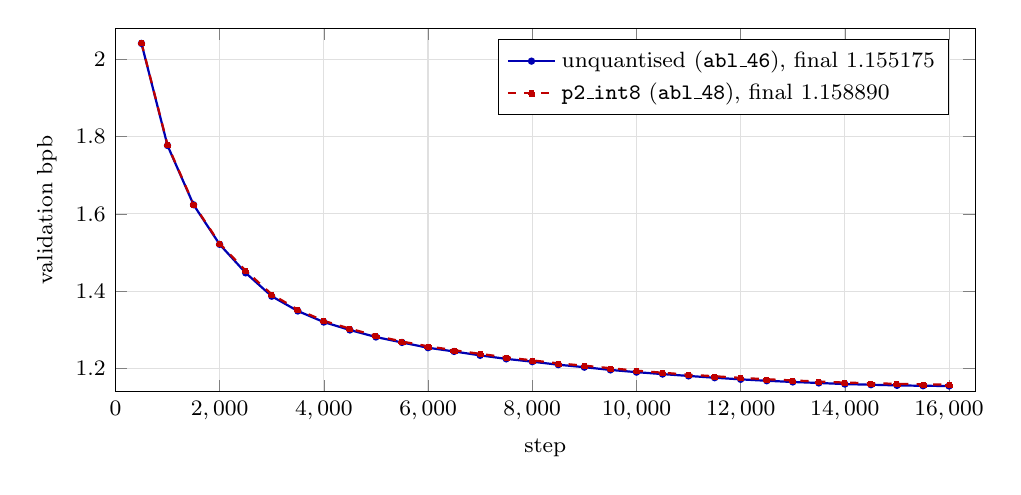
\begin{tikzpicture}
\begin{axis}[width=12.5cm,height=6.2cm,xlabel={step},ylabel={validation bpb},xmin=0,xmax=16500,ymin=1.14,ymax=2.08,
  legend pos=north east,legend cell align=left,grid=major,grid style={black!12},tick label style={font=\footnotesize},label style={font=\footnotesize},
  legend style={font=\footnotesize},scaled x ticks=false,xticklabel style={/pgf/number format/1000 sep={,}}]
\addplot[blue!70!black,thick,mark=*,mark size=0.9pt] coordinates {(500,2.040832) (1000,1.776875) (1500,1.623594) (2000,1.521324) (2500,1.447563) (3000,1.387140) (3500,1.349000) (4000,1.320404) (4500,1.299948) (5000,1.281772) (5500,1.267666) (6000,1.254039) (6500,1.244459) (7000,1.234356) (7500,1.225330) (8000,1.218026) (8500,1.210181) (9000,1.203784) (9500,1.196733) (10000,1.190968) (10500,1.185965) (11000,1.181152) (11500,1.176543) (12000,1.172354) (12500,1.168671) (13000,1.165571) (13500,1.162982) (14000,1.160156) (14500,1.158426) (15000,1.156762) (15500,1.155690) (16000,1.155175)};
\addlegendentry{unquantised (\code{abl\_46}), final 1.155175}
\addplot[red!75!black,thick,dashed,mark=square*,mark size=0.9pt] coordinates {(500,2.042345) (1000,1.778489) (1500,1.625179) (2000,1.523535) (2500,1.453096) (3000,1.392056) (3500,1.352562) (4000,1.323561) (4500,1.303378) (5000,1.285084) (5500,1.270053) (6000,1.257795) (6500,1.247624) (7000,1.238201) (7500,1.229284) (8000,1.221387) (8500,1.213690) (9000,1.207693) (9500,1.201220) (10000,1.194780) (10500,1.189506) (11000,1.184390) (11500,1.180368) (12000,1.176174) (12500,1.172609) (13000,1.169557) (13500,1.166627) (14000,1.164038) (14500,1.162242) (15000,1.160825) (15500,1.159512) (16000,1.158890)};
\addlegendentry{\code{p2\_int8} (\code{abl\_48}), final 1.158890}
\end{axis}
\end{tikzpicture}\hspace{0.6cm}%
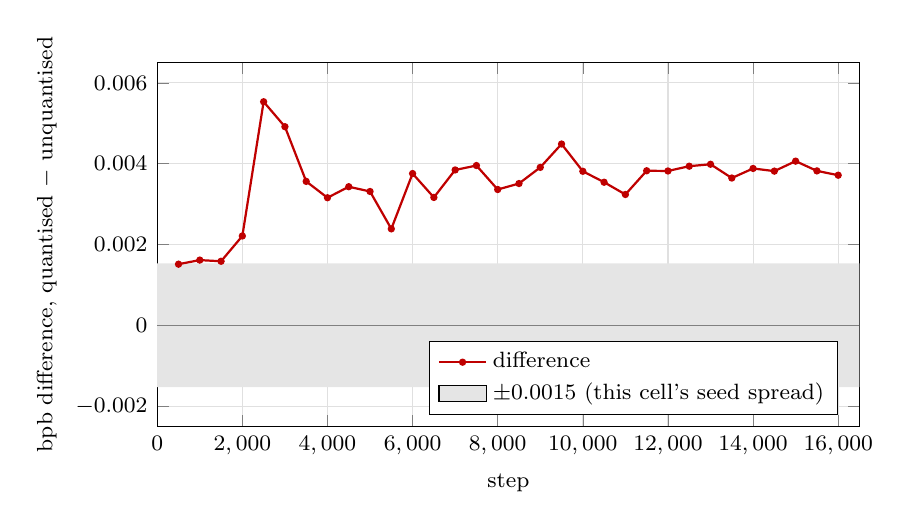
\begin{tikzpicture}
\begin{axis}[width=10.5cm,height=6.2cm,xlabel={step},ylabel={bpb difference, quantised $-$ unquantised},xmin=0,xmax=16500,ymin=-0.0025,ymax=0.0065,
  grid=major,grid style={black!12},tick label style={font=\footnotesize},label style={font=\footnotesize},scaled x ticks=false,scaled y ticks=false,
  yticklabel style={/pgf/number format/fixed,/pgf/number format/precision=3},xticklabel style={/pgf/number format/1000 sep={,}},legend style={font=\footnotesize},legend pos=south east,legend cell align=left]
\addplot[fill=black!10,draw=none,forget plot] coordinates {(0,-0.00153) (16500,-0.00153) (16500,0.00153) (0,0.00153)} \closedcycle;
\addplot[black!50,thin,forget plot] coordinates {(0,0) (16500,0)};
\addplot[red!75!black,thick,mark=*,mark size=0.9pt] coordinates {(500,0.001513) (1000,0.001614) (1500,0.001585) (2000,0.002211) (2500,0.005533) (3000,0.004916) (3500,0.003562) (4000,0.003157) (4500,0.003430) (5000,0.003312) (5500,0.002387) (6000,0.003756) (6500,0.003165) (7000,0.003845) (7500,0.003954) (8000,0.003361) (8500,0.003509) (9000,0.003909) (9500,0.004487) (10000,0.003812) (10500,0.003541) (11000,0.003238) (11500,0.003825) (12000,0.003820) (12500,0.003938) (13000,0.003986) (13500,0.003645) (14000,0.003882) (14500,0.003816) (15000,0.004063) (15500,0.003822) (16000,0.003715)};
\addlegendentry{difference}
\addlegendimage{area legend,fill=black!10,draw=none}
\addlegendentry{$\pm0.0015$ (this cell's seed spread)}
\end{axis}
\end{tikzpicture}
\end{center}

\section*{Long-run results (48K steps)}
The quantised variant (\code{p2\_int8}) of 3.2 $+$TV at 48K steps, warmup and cosine schedule stretched to 48K, run on nebius
(\code{exp\_n\_abl\_47\_B48k\_light\_lmfrozeng\_n2\_tau0p5\_tv10\_tph128\_seed1\_p2int8}; training time 3.67\,h):
final validation bpb \textbf{1.123253} at step 48,000 and best \textbf{1.122593} at step 47,000, over 96 evaluations with the fixed evaluation
(batch 48 $\times$ 100 steps, the first 12 rows skipped), the protocol of every other number in this document.
The curve falls from 1.439334 at step 4,000 to 1.185099 at 16,000 and 1.125973 at 40,000, and is flat from step 43,000:
its last eleven evaluations lie within $0.0009$ (1.122593 to 1.123513), with no divergence.
\textbf{Against the vanilla dense FFN at 48K} (untied, same fixed evaluation; \code{exp\_n\_0177\_vanilla48k\_corrected}, final 1.115420, best 1.115092 at step 47,500)
the quantised variant is $+0.007501$ bpb above best against best and $+0.007833$ final against final.
\end{document}
